\section{Metrics}
\label{sec:Solution} 

%
%\begin{figure}[H]
	%\centering
		%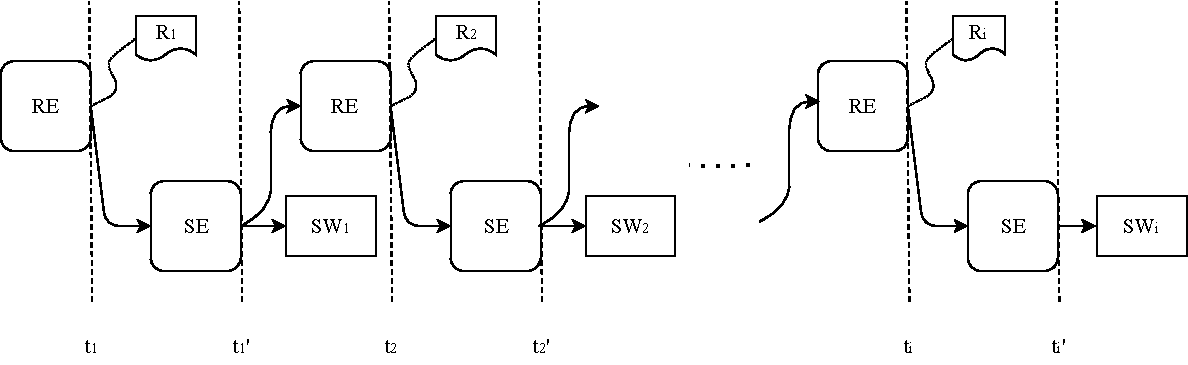
\includegraphics[width=0.8\textwidth,height=2in]{MetricsDiag.pdf}
	%\caption{Requirements engineering and development processes}
	%\label{fig:Metrics_shot}
%\end{figure}

%In these metrics we consider a maturity of requirements as a characteristic of the quality.
%
\autoref{fig:Metrics_shot} provides a graphical explanation of the metrics. The workflow is divided into requirements engineering (RE) 
and system implementation (SI) processes' iterations along the time line: $t_{1},t_{2},...,t_{i}$ - 
instants of time for RE phases (RE iteration); $t_{1}',t_{2}',...,t_{i}'$ - 
instants of time for implementation process based on the provided requirements (SI iteration).
The output of every RE iteration is RE artifact (a document with the full set of the requirements) - depicted as $R_{1},R_{2},...,R_{i}$; and every SI phase results into SI artifact, 
e.g., software architecture (shown as SW), till the end of the SI phase, which leads to the release of a product and end of the project. 

The input for the first iteration of RE process is a "raw" requirements. During the RE phase, the requirements become elaborated (changed with respect to a project's demands); the result of this process is a corrected RE artifact, that is an input 

\newpage
\hfill \break

\vspace{5.4cm}

to the next stage (SI). Therefore, we consider the initial RE artifact as a document \textit{$\mu(R_{j})=0$}. 
 
\subsection{Metrics for a full set of requirements}

We defined, that every RE artifact has its index of maturity. The range of this metric varies from 0 to 1: 0 means ``bad'' and 1 indicates ``good'' quality.
The maturity index is inferred from a number of iterations (a certain amount of changes applied to requirements' document) and the time spent for RE and implementation process.
The more mature a requirement is, the less changes (iterations) the artifact requires, and the shorter the time for the development process. 
\textsl{Thus, the better quality of the requirements: the higher index of the requirements maturity} (\autoref{eqn:maturity_ind}). 

In \autoref{eqn:maturity_ind}, the maturity index reflects, how far the considered requirements with the certain maturity parameters (presented as a sum of the metrics for the full set of the requirements - $\sum\mu_{n}(R_{j})$) from their ``good'' state (defined as 1)

  \begin{equation}\label{eqn:maturity_ind}
\textrm{\textit{maturity index}} = \frac{1}{\sum_{n=1}^{2}\mu_{n}(R_{j})}
	\end{equation}

where $(R_{j}$) is a considered RE artifact; $j$ is an starting iteration for calculation.
%where $\mu(R_{j})$ is a calculated number of the iterations for a considered RE artifact $(R_{j}$); $j$ is an initial iteration for calculation.

Consequently, to calculate the \textit{maturity index} of the requirements, the following metrics should be determined:

 \begin{equation}\label{eqn:mu1}
\mu_{1}(R_{j}) = i-j
	\end{equation}
	
\textrm{end of the number of iterations for the requirements} $R_{j}$;

 \begin{equation}\label{eqn:mu2}
\mu_{2}(R_{j}) = t_{i}\acute{}-t_{j}    
 \end{equation}

\textrm{amount of time (in hours) between initial and the last phases of the development process applying the requirements} $R_{j}$;

%\begin{equation}\label{eqn:mu3}
%\mu_{3}(R_{j}) = \displaystyle\sum_{j} t_{j+1}-t_{j}\acute{}
%\end{equation}
%
%,\textrm{total amount of time (in hours) required for SI process};


%(here, along with requirements' maturity, we can also talk about such quality criterion as the requirements' comprehensibility);
%$\mu_{4} = \displaystyle\sum_{j} (t_{j+1}-t_{j}\acute{} + p_{j}*(t_{j}\acute{} - t_{j}))$

\subsection{Metrics for a single requirement}


